\chapter{LAPORAN}
\section{TUGAS TEORI}
\begin{itemize}
	\item Fungsi\\
	Fungsi merupakan sekumpulan kode blok yang disusun secara terorganisir dan dapat digunakan kembali di kemudian untuk membuat sebuah tindakan. 
	\begin{enumerate}
	\item Inputan Fungsi\\
		Untuk membuat inputan fungsi, terdapat beberapa aturan yang harus dipatuhi, di antaranya yaitu :\\
		\begin{enumerate}
		\item Penulisan fungsi dimulai dengan def sebagai kata kunci, kemudian diikuti oleh nama fungsi itu sendiri disertai dengan tanda kurung ()
		\item Setiap parameter dalam fungsi tersebut dituliskan di dalam kurung tersebut, di dalamnya juga dapat dilakukan penentuan atau pengaturan terhadap variabel di dalamnya.
		\item Blok kode yang dituliskan pada fungsi selalu diikuti dengan titik dua (:) dan diikuti oleh indentasi setelahnya.\\
		Berikut ini merupakan contoh pembuatan inputan fungsi yang benar
		        \begin{figure}[H]
				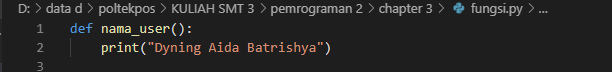
\includegraphics[width=20cm]{figures/1184030/fungsi/input.PNG}
				\centering
				\caption{inputan fungsi}
				\end{figure}
		\end{enumerate}
		\item Berikut ini merupakan cara pemanggilan kode fungsi
		        \begin{figure}[H]
				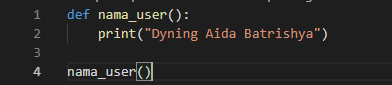
\includegraphics[width=20cm]{figures/1184030/fungsi/panggil.PNG}
				\centering
				\caption{pemanggilan fungsi}
				\end{figure}
				Tata cara pemanggilan fungsi dapat dilakukan dengan menuliskan nama dari fungsi yang telah dibuat sebelumnya yang kemudian diikuti dengan tanda kutung (()) yang diikuti dengan menuliskan parameter yang terdapat di dalamnya.
		\item Contoh kode program sederhana yang menggunakan fungsi :\\
		        \begin{figure}[H]
				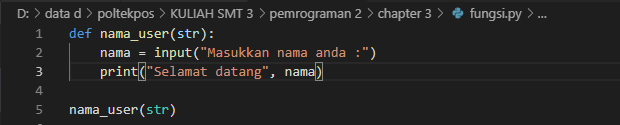
\includegraphics[width=20cm]{figures/1184030/fungsi/program.PNG}
				\centering
				\caption{contoh program sederhana yang menggunakan fungsi}
				\end{figure}
	\end{enumerate}
	\item Pengertian Paket Library dan Cara penggunaannya
	class digunakan untuk membuat struktur data pengguna yang berisikan tentang informasi terhadap suatu objek yang akan didefinisikan. contoh pemakaian class yaitu 
	\item Pengertian kelas, objek, atribut, dan method
	\begin{enumerate}
	    \item Pengertian Kelas\\
	    Kelas adalah blue print atau prototipe dari suatu kelas yang mendefinisikan atribut dari suatu objek
	    \item Pengertian Objek\\
	    Objek merupakan instansiasi atau perwujudan suatu class, bisa disebut juga bahwa objek merupakan hasil atau barang jadinya
	    \item Pengertian Atribut\\
	    Suatu data yang merupakan anggota dari sebuah variabel yang diakses dengan menggunakan notasi titik.
	    \item Pengertian Method\\
	    Method merupakan suatu pendefinisian fungsi dari suatu class.
	\end{enumerate}
	\item Cara pemanggilan library melalui instansiasi\\
	Instansiasi adalah cara pemanggilan instance atau objek dari suatu kelas yang telah dibuat sebelumnya.
	\item Contoh pemakaian paket dengan perintah from kalkulator import\\
	Berikut ini merupakan contoh pembuatan paket kalkulator
	\lstinputlisting[language=Python]{src/kalkulator.py}
	Cara pemanggialan perintah from kalkulator import
	\lstinputlisting[language=Python]{src/call.py}
	\item Kode ketika pemanggilan paket fungsi dalam sebuah library yang sama\\
        \begin{enumerate}
	    \item Buat kelas yang berisikan kumpulan fungsi di dalamnya
	    \item Panggil dengan menggunakan kata kunci "import from (nama fungsi)". Berikut ini merupakan contohnya :\\ Contoh pembuatan paket fungsi
	    \lstinputlisting[language=Python]{src/kelasfungsi.py}
	    Contoh pemanggilan paket fungsi
	    \lstinputlisting[language=Python]{src/panggil.py}
	\end{enumerate}
	\item Kode ketika pemanggilan paket fungsi dalam sebuah library yang berbeda
		Untuk pemanggilan paket fungsi yang berbeda folder, maka harus dituliskan nama folder yang menyimpan paket fungsi tersebut dahulu sebelum mengimport fungsinya
\end{itemize}
\section{KETERAMPILAN}
1. \lstinputlisting[language=Python]{src/NPM1.py}
2. \lstinputlisting[language=Python]{src/NPM2.py}
3. \lstinputlisting[language=Python]{src/NPM3.py}
4. \lstinputlisting[language=Python]{src/NPM4.py}
5. \lstinputlisting[language=Python]{src/NPM5.py}
6. \lstinputlisting[language=Python]{src/NPM6.py}
7. \lstinputlisting[language=Python]{src/NPM7.py}
8. \lstinputlisting[language=Python]{src/NPM8.py}
9. \lstinputlisting[language=Python]{src/NPM9.py}
10. \lstinputlisting[language=Python]{src/NPM10.py}
11. \lstinputlisting[language=Python]{src/lib3.py}
12. \lstinputlisting[language=Python]{src/main.py}
    \lstinputlisting[language=Python]{src/kelas3lib.py}
\section{KETERAMPILAN PENANGANAN ERROR}
\begin{enumerate}
\item peringatan error pada praktek ketiga dan penjelasan penanganan error tersebut.\\
Peringatan error yang muncul salah satunya yaitu seperti gambar di bawah ini :\\
\lstinputlisting[language=Python]{src/penanganan.py}
		Cara penanganan yang digunakan untuk mengatasi error tersebut yaitu dengan memberikan try untuk menghasilkan/mencetak fungsi sebelumnya, kemudian jika parameter yang ditangkap tidak sesuai maka, program akan mengeksekusi exception dan mencetak peringatannya.
\end{enumerate}
\section{SCAN PLAGIARISME}
                \begin{figure}[H]
				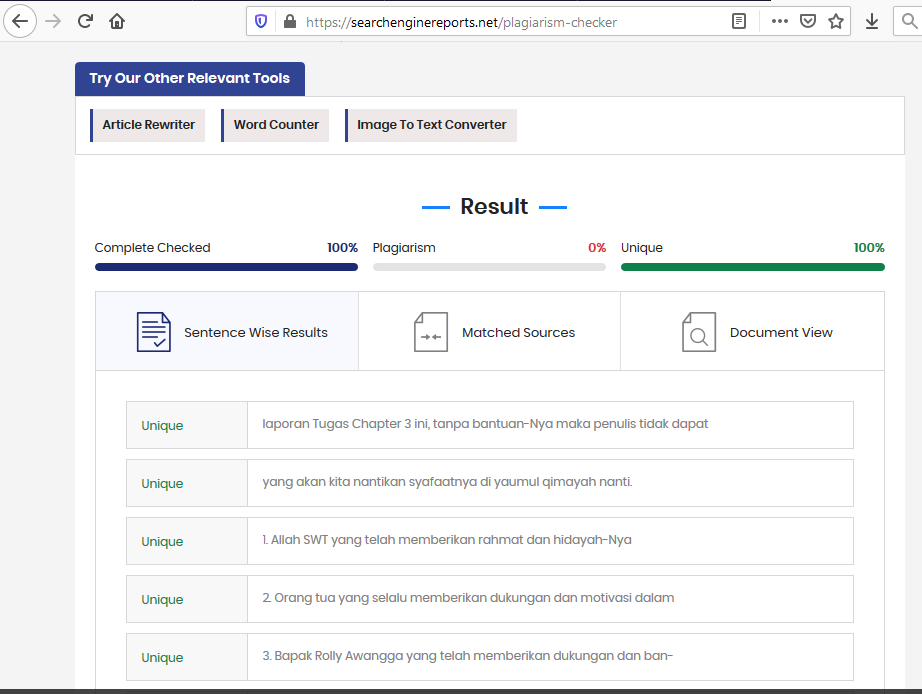
\includegraphics[width=20cm]{figures/1184030/fungsi/plagiarisme.PNG}
				\centering
				\caption{hasil scan plagiarisme}
				\end{figure}